\section{Precision of Indoor Location}\label{sec:estimoteprecision}
Another core part of our system is indoor location. 
For the ``point-to-select'' part of our system to work as intended, we need high indoor precision. 
In \Cref{sec:designindoorlocation} we mentioned that Estimote claims the accuracy to be \num{0.5}-\num{1} meters.
In this section we test if that is actually the case, or even if we can achieve better results than that. 

Different tests were conducted to explore the changes caused by change in room size, change in broadcasting interval, broadcasting power, standing still versus moving and using the system outdoors.

\subsection{Changing Room Size & Stationary vs. Moving}
For this test the objective was to test how accurate the location system was in two rooms of different sizes.

\subsubsection*{Setup}
To be able to scale the room we created the test room inside of a larger room by arranging tables in a square to represent walls and then adding a chair in the middle of each of these walls to be able to install the Estimote beacons in a proper height.
A drawing of this setup is shown in \cref{fig:precisiontest:illustration} and a photo of it is shown in \cref{fig:precisiontest:chairs}.

\begin{figure}[!htb]
    \centering
    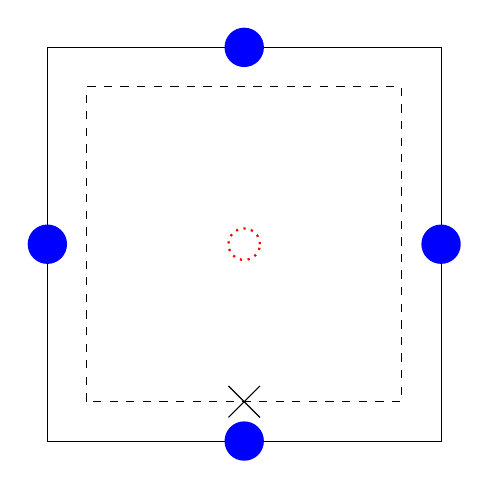
\begin{tikzpicture}

    \draw (0,0) rectangle (5,5); % Outline of room
    
    \draw[red,thick,dotted] (2.5,2.5) circle (0.2); % Phone location
    
    \fill[blue!100!] (2.5, 0) circle (0.25); % Beacon location - Bottom
    \fill[blue!100!] (5, 2.5) circle (0.25); % Beacon location - Right
    \fill[blue!100!] (2.5, 5) circle (0.25); % Beacon location - Top
    \fill[blue!100!] (0, 2.5) circle (0.25); % Beacon location - Left
    
    % Walking path
    \draw[dashed] (0.5,0.5) rectangle (4.5,4.5);
    
    % Start / stop point of walking path
    \draw (2.3,0.7) -- (2.7,0.3);
    \draw (2.3,0.3) -- (2.7,0.7);
    
    \end{tikzpicture}
    \caption{Illustration of room used for indoor location precision test.}
\label{fig:precisiontest:illustration}
\end{figure}

The dotted red circle in the center of \cref{fig:precisiontest:illustration} represents the phone's location in the tests where it remained stationary.
The blue circles in the sides represent Estimote beacons.
The dashed square represents the path that a person walked along whilst holding the phone, and the X represents the point where the path began and ended.

The setup consisted of four beacons, one on each wall, each using the recommended settings\cite{estimote:settings}:
\begin{description}
    \item[Broadcasting Power]{4 dBm}
    \item[Advertising Interval]{200 ms}
    \item[Smart Power Mode]{Enabled}
    \item[Basic Power Mode]{Disabled}
\end{description}

\begin{figure}[!htb]
    \centering
    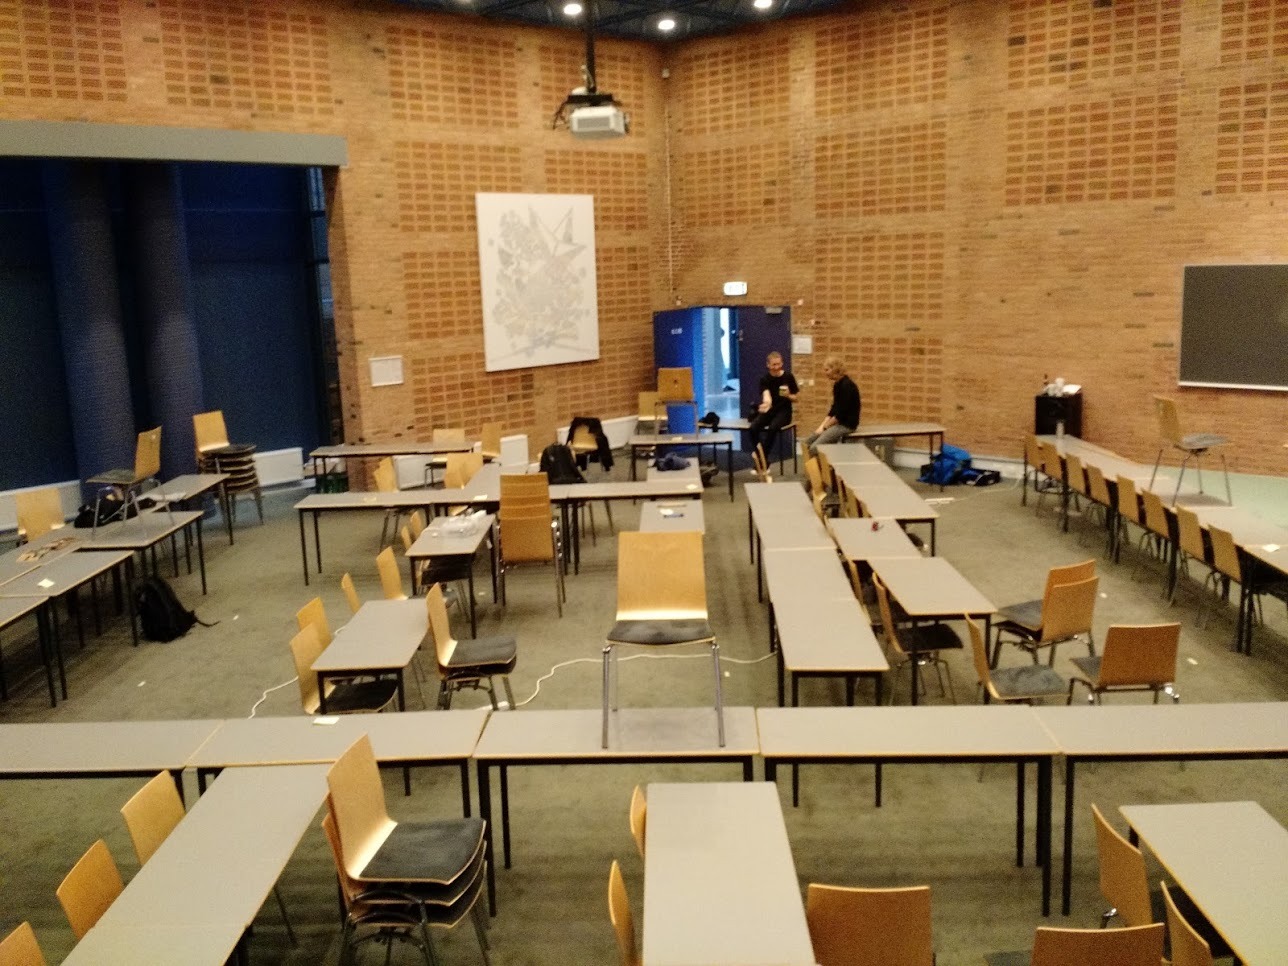
\includegraphics[width=\textwidth]{precision-test-photo.jpg}
    \caption{Picture of the room built with chairs.}
\label{fig:precisiontest:chairs}
\todo[author=Kasper]{We should probably edit the photo and highlight important parts like the chairs with beacons, otherwise these image is too cluttered.}
\end{figure}

\subsubsection*{Procedure}
The first tests were conducted by creating a room of size $5\times 5$ meters and then placing the phone on a table in center of the room.
Position data was then logged on the phone for a duration of one minute.
This was done 4 times and then a fifth time where the duration was increased to two minutes.

Next a person held the phone in his hand parallel to the floor and followed the path specified by the dashed line in \cref{fig:precisiontest:illustration}. He went around the room along this path two times.

Afterwards the room size was increased to $8\times 8$ meters and the tests repeated.

The tests conducted are shown in \cref{table:precisiontest:roomsize}.

\begin{table}[h!]
\centering
\begin{tabular}{|l|l|l|l|}
\hline
Room Size  & Phone Position & Duration & Count \\ \hline
$5\times 5$ meters & Center         & 1min     & 4     \\ \hline
$5\times 5$ meters & Center         & 2min     & 1     \\ \hline
$5\times 5$ meters & Moving         & NA       & 3     \\ \hline
$8\times 8$ meters & Center         & 1min     & 3     \\ \hline
$8\times 8$ meters & Center         & 2min     & 1     \\ \hline
$8\times 8$ meters & Moving         & NA       & 3     \\ \hline
\end{tabular}
\caption{Tests conducted with varying room size.}
\label{table:precisiontest:roomsize}
\end{table}

\subsection{Changing Beacon Configuration}
For this test the objective was to test how accurate the location system was in a single room using settings on the beacons.

\subsubsection*{Setup}
The tests were conducted in a room of size $490\times 995$cm using four beacons, one on each wall.

\subsubsection*{Procedure}
The tests conducted in this room had the phone placed on a table in the center of the room and logging position data for a duration of one minute.
This was done three times and then the settings of the beacons were changed.

The settings are shown in \cref{table:precisiontest:settings}.

\begin{table}[h!]
\centering
\begin{tabular}{l|l}
Advertising Interval & Broadcasting Power \\ \hline
200 ms               & 4 dBm              \\ 
200 ms               & -20 dBm            \\ 
200 ms               & -12 dBm            \\ 
200 ms               & -4 dBm             \\ 
100 ms               & 4 dBm              \\ 
\end{tabular}
\caption{Tests conducted with varying settings on the beacons.}
\label{table:precisiontest:settings}
\end{table}

\subsection{Outdoors}
For this test the objective was to test how accurate the location system was outdoors.

\subsubsection*{Setup}
To construct a room outdoors we mounted the beacons on street lamps in a parking lot to form a room of size $1790\times 1790$ cm. The beacons used the recommended settings\cite{estimote:settings}:
\begin{description}
    \item[Broadcasting Power]{4 dBm}
    \item[Advertising Interval]{200 ms}
    \item[Smart Power Mode]{Enabled}
    \item[Basic Power Mode]{Disabled}
\end{description}

\subsubsection*{Procedure}
The tests were conducted by placing the phone on the ground in the center of the room and logging position data for a duration of one minute.
This was done three times.

\subsection{Precision of Indoor Location Conclusion}
From the results, we can conclude that... \todo[author=Thalley]{Write conclusion of precision test based on results}

